
%\documentclass[mathserif]{beamer}
\documentclass[handout]{beamer}
%\usetheme{Goettingen}
%\usetheme{Warsaw}
\usetheme{Singapore}



%\usetheme{Frankfurt}
%\usetheme{Copenhagen}
%\usetheme{Szeged}
%\usetheme{Montpellier}
%\usetheme{CambridgeUS}
%\usecolortheme{}
%\setbeamercovered{transparent}
\usepackage[english, activeacute]{babel}
\usepackage[utf8]{inputenc}
\usepackage{amsmath, amssymb}
\usepackage{dsfont}
\usepackage{graphics}
\usepackage{cases}
\usepackage{graphicx}
\usepackage{pgf}
\usepackage{epsfig}
\usepackage{amssymb}
\usepackage{multirow}	
\usepackage{amstext}
\usepackage[ruled,vlined,lined]{algorithm2e}
\usepackage{amsmath}
\usepackage{epic}
\usepackage{epsfig}
\usepackage{fontenc}
\usepackage{framed,color}
\usepackage{palatino, url, multicol}
%\algsetup{indent=2em}
\newcommand{\factorial}{\ensuremath{\mbox{\sc Factorial}}}
\newcommand{\BIGOP}[1]{\mathop{\mathchoice%
{\raise-0.22em\hbox{\huge $#1$}}%
{\raise-0.05em\hbox{\Large $#1$}}{\hbox{\large $#1$}}{#1}}}
\newcommand{\bigtimes}{\BIGOP{\times}}
\vspace{-0.5cm}
\title{Natural Language Processing \\ Linear Models}
\vspace{-0.5cm}
\author[Felipe Bravo Márquez]{\footnotesize
%\author{\footnotesize  
 \textcolor[rgb]{0.00,0.00,1.00}{Felipe Bravo-Marquez}} 
  
 

\date{\today}

\begin{document}
\begin{frame}
\titlepage


\end{frame}



\begin{frame}{Supervised Learning}
\begin{scriptsize}
\begin{itemize}
\item The essence of supervised machine learning is the creation of mechanisms that can look at examples and produce generalizations. \cite{goldberg2017neural}
\item We design an algorithm whose input is a set of labeled examples, and
its output is a function (or a program) that receives an instance and produces the desired label.
\item Example: if the task is to distinguish from spam and not-spam email, the labeled examples are emails labeled as spam and emails labeled as not-spam.
\item It is expected that the resulting function will produce correct label
predictions also for instances it has not seen during training.
\item This approach differs from designing an algorithm to perform the task (e.g., manually designed rule-based systems).
\end{itemize}


\end{scriptsize}
\end{frame}


\begin{frame}{Parameterized Functions}
\begin{scriptsize}
\begin{itemize}
\item Searching over the set of all possible functions is a very hard (and rather ill-defined) problem. \cite{goldberg2017neural}
\item We often restrict ourselves to search over specific families of functions.
\item Example: the space of all linear functions with $d_{in}$ inputs and $d_{out}$ outputs, 
\item Such families of functions are called \textbf{hypothesis classes}. 
\item By restricting ourselves to a specific hypothesis class, we are injecting the learner with \textbf{inductive bias}.
\item Inductive bias: a set of assumptions about the form of the desired solution.
\item Some hypothesis classes facilitate efficient procedures for searching for the solution. \cite{goldberg2017neural}
\end{itemize}


\end{scriptsize}
\end{frame}


\begin{frame}{Linear Models}
\begin{scriptsize}
\begin{itemize}
\item One common hypothesis class is that of high-dimensional linear function:
\begin{equation}
\begin{split}
f(\vec{x}) = \vec{x} \cdot W + \vec{b}\\
\vec{x} \in  \mathcal{R}^{d_{in}} & \quad W \in  \mathcal{R}^{d_{in}\times d_{out}} \quad \vec{b} \in  \mathcal{R}^{d_{out}}
\end{split}
\end{equation}
\item The vector $\vec{x}$ is the input to the function.
\item The matrix $W$ and the vector $\vec{b}$ are the \textbf{parameters}.

\item The goal of the learner is to set the values of the parameters $W$ and $\vec{b}$ such that the function behaves as intended on a collection of input values $\vec{x}_{1:k} = \vec{x}_1,\dots,\vec{x}_k$ and the corresponding desired outputs $\vec{y}_{1:k} = \vec{y}_1,\dots,\vec{y}_k$

\item The task of searching over the space of functions is thus reduced to one of searching over the space of parameters. \cite{goldberg2017neural}

\end{itemize}


\end{scriptsize}
\end{frame}


\begin{frame}{Example: Language Detection}
\begin{scriptsize}
\begin{itemize}
\item Consider the task of distinguishing documents written in English from documents written in German.
\item This is a binary classifcation problem 
\begin{equation}
\begin{split}
f(\vec{x}) = \vec{x} \cdot \vec{w} + b\\
\end{split}
\end{equation}
 $d_{out}=1$, $\vec{w}$ is a vector, and $b$ is a scalar. 

 \item The range of the linear function in is $[-\infty,\infty]$.
 \item In order to use it for binary classification, it is common to pass the output of $f(x)$ through the $sign$ function, mapping negative values to -1 (the negative class) and non-negative values to +1 (the positive class).
\end{itemize}


\end{scriptsize}
\end{frame}


\begin{frame}{Example: Language Detection}
\begin{scriptsize}
\begin{itemize}

\item Letter frequencies make for quite good predictors (features) for this task.
\item Even more informative are counts of letter bigrams, i.e., pairs of consecutive letters.
\item One may think that words will also be good predictors i.e., using a bag of word representation of documents.
\item Letters, or letter-bigrams are far more robust.
\item We are likely to encounter a new document without any of the words we observed in the training set.
\item While a document without any of the distinctive letter-bigrams is significantly less likely. \cite{goldberg2017neural}
\end{itemize}


\end{scriptsize}
\end{frame}



\begin{frame}{Example: Language Detection}
\begin{scriptsize}
\begin{itemize}
\item We assume we have an alphabet of 28 letters (a–z, space, and a special symbol for all other characters including digits, punctuations, etc.)
\item Documents are represented as $28\times28$ dimensional vectors $\vec{x} \in \mathcal{R}^{784}$.
\item Each entry $\vec{x}_{[i]}$  represents a count of a particular letter combination in the document, normalized by the document's length.
\item For example, denoting by $\vec{x}_{ab}$ the entry of $\vec{x}$ corresponding to the letter bigram $ab$:
\begin{equation}
 x_{ab}= \frac{\#ab}{|D|}
\end{equation}
where $\#ab$ is the number of times the bigram $ab$ appears in the document, and $|D|$ is the total number of bigrams in the document (the document’s length).


\end{itemize}


\end{scriptsize}
\end{frame}




\begin{frame}{Example: Language Detection}


\begin{figure}[htb]
	\centering
	 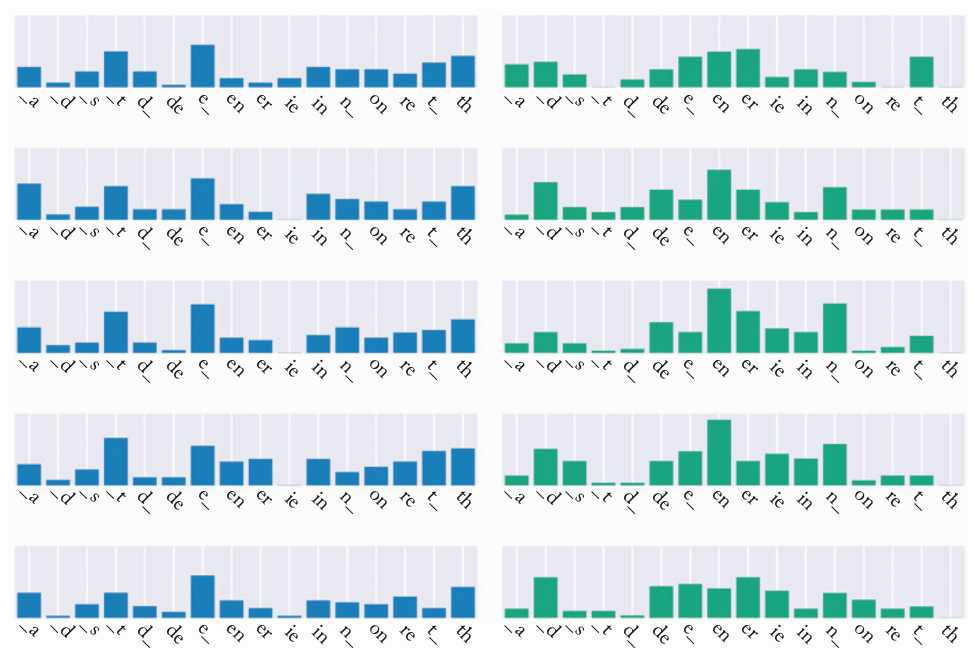
\includegraphics[scale=0.27]{pics/langbigrams.png}
\end{figure}

\scriptsize{Character-bigram histograms for documents in English (left, blue) and German(right,green). Underscores denote spaces. Only the top frequent character-bigrams are showed.}

\footnotetext{Source:\cite{goldberg2017neural}}

\end{frame}


\begin{frame}{Example: Language Detection}
\begin{scriptsize}
\begin{itemize}
\item Previous figure showed clear patterns in the data, and, given a new item, such as:

\begin{figure}[htb]
	\centering
	 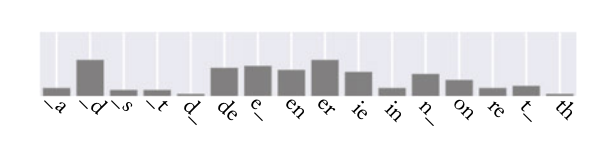
\includegraphics[scale=0.4]{pics/langbigramstest.png}
\end{figure}

\item We could probably tell that it is more similar to the German group than to the English one (observe the frequency of ``th'' and ``ie'').

\item We can't use a single definite rule such as ``if it has th its English'' or ``if it has ie its German''.
\item While German texts have considerably less ``th'' than English, the ``th'' may and does occur in German texts, and similarly the ``ie'' combination does occur in English.


\end{itemize}


\end{scriptsize}
\end{frame}



\begin{frame}{Example: Language Detection}
\begin{scriptsize}
\begin{itemize}
\item The decision requires weighting different factors relative to each other.
\item We can formalize the problem in a machine-learning setup using a linear model:
\begin{equation}
\begin{split}
\hat{y} \quad = sign(f(\vec{x})) & = sign(\vec{x}\cdot \vec{w} + b) \\ 
& = sign(\vec{x}_{aa}\times \vec{w}_{aa}+ \vec{x}_{ab}\times \vec{w}_{ab}+ \vec{x}_{ac}\times \vec{w}_{ac} \dots +b)
\end{split}
\end{equation}
\item A document will be considered English if $f(\vec{x}) \geq 0$  and as German otherwise.
\end{itemize}

\begin{block}{Intuition}
\begin{enumerate}
\item Learning should assign large positive values to $\vec{w}$ entries associated with letter pairs that are much more common in English than in German (i.e., ``th'').
\item It should also assign negative values to letter pairs that are much more common in German than in English (``ie'', ``en'').
\item Finally, it should assign  values around zero to letter pairs that are either common or rare in both languages.
\end{enumerate}
\end{block}
\end{scriptsize}
\end{frame}




\begin{frame}{Log-linear Binary classifcation}
\begin{scriptsize}
\begin{itemize}
\item The output $f(\vec{x})$ is in the range $[-\infty,\infty]$ , and we map it to one of two classes $\{-1,+1\}$ using the $sign$ function.
\item This is a good fit if all we care about is the assigned class.
\item We may be interested also in the confidence of the decision, or the probability that the classifier assigns to the class.
\item An alternative that facilitates this is to map instead to the range $[0,1]$, by pushing the output through a squashing function such as the sigmoid $\sigma(x)$:
\begin{equation}
\sigma(x) = \frac{1}{1+e^{-x}}  
\end{equation}
resulting in: 
\begin{equation}
\hat{y}=\sigma(f(\vec{x})) = \frac{1}{1+e^{-\vec{x}\cdot \vec{w}+b}}  
\end{equation}

\end{itemize}
\end{scriptsize}
\end{frame}


\begin{frame}{The Sigmoid function}
\begin{figure}[htb]
	\centering
	 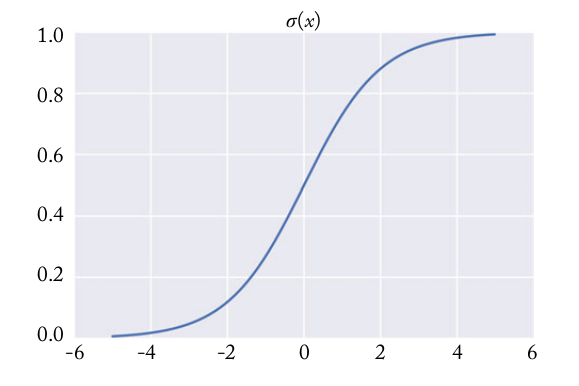
\includegraphics[scale=0.5]{pics/sigmoid.png}
\end{figure}
\end{frame}



\begin{frame}{The Sigmoid function}

\begin{scriptsize}
\begin{itemize}
\item The sigmoid function is is monotonically increasing, and maps values
to the range $[0, 1]$, with $0$ being mapped to $\frac{1}{2}$.
\item When used with a suitable loss function (discussed later) the binary predictions made through the log-linear model can be interpreted as class membership probability estimates:
\begin{equation}
 \sigma(f(\vec{x})) = P(\hat{y} = 1| \vec{x}) \quad \text{of $\vec{x}$ belonging to the positive class.}
\end{equation}
\item We also get $P(\hat{y} = 0| \vec{x}) = 1 - P(\hat{y} = 1| \vec{x}) = 1 -  \sigma(f(\vec{x}))$
\item The closer the value is to $0$ or $1$ the more certain the model is in its class membership prediction, with the value of $0.5$ indicating model uncertainty.
\end{itemize}
\end{scriptsize}
\end{frame}




\begin{frame}{Multi-class Classification}

\begin{scriptsize}
\begin{itemize}
\item Most classification problems are of a multi-class nature: examples are assigned to one of $k$ different classes.
\item Example: we are given a document and asked to classify it into one of six possible languages: English, French, German, Italian, Spanish, Other.
\item Possible solution: consider six weight vectors $\vec{w}_{EN}$,$\vec{w}_{FR},\dots$ and biases (one for each language).
\item Predict the language resulting in the highest score:
\begin{equation}
 \hat{y} = f(\vec{x}) = \operatorname{argmax}_{L \in \{ EN,FR,GR,IT,SP,O \}} \quad \vec{x}\cdot \vec{w}_L+ b_{L}
\end{equation}
\end{itemize}
\end{scriptsize}
\end{frame}



\begin{frame}{Multi-class Classification}

\begin{scriptsize}
\begin{itemize}
\item The six sets of parameters $\vec{w}_L \in  \mathcal{R}^{784}$ and $b_L$  can be arranged as a matrix $W \in \mathcal{R}^{784\times6}$ and vector $\vec{b} \in \mathcal{R}^6$ , and the equation re-written as:
\begin{equation}
 \begin{split}
  \vec{\hat{y}} = f(\vec{x}) = \quad & \vec{x} \cdot W + \vec{b}\\
   \text{prediction} = \hat{y} = \quad  & \operatorname{argmax}_i \vec{\hat{y}}_{[i]} 
 \end{split}
\end{equation}

\item Here $\vec{\hat{y}} \in \mathcal{R}^6$ is a vector of the scores assigned by the model to each language, and we again determine the predicted language by taking the argmax over the entries of $\vec{\hat{y}}$.

\end{itemize}
\end{scriptsize}
\end{frame}


\begin{frame}{Representations}

\begin{scriptsize}
\begin{itemize}
\item Consider the vector $\vec{\hat{y}}$  resulting from applying a trained model to a document.
\item The vector can be considered as a representation of the document.
\item It captures the properties of the document that are important to us:  the scores of the different languages.
\item The representation $\vec{\hat{y}}$  contains strictly more information than the prediction $\operatorname{argmax}_i \vec{\hat{y}}_{[i]} $.
\item Example: $\vec{\hat{y}}$ can be used to distinguish documents in which the main language is German, but which also contain a sizeable amount of French words.
\item Clustering documents based on $\vec{\hat{y}}$ could help to discover documents written in regional dialects, or by multilingual authors.


\end{itemize}
\end{scriptsize}
\end{frame}


\begin{frame}{Representations}

\begin{scriptsize}
\begin{itemize}
\item The vectors $\vec{x}$ containing the normalized letter-bigram counts for the documents are also representations of the documents.
\item Arguably containing a similar kind of information to the vectors $\vec{\hat{y}}$. 
\item However, the representations in  $\vec{\hat{y}}$ is more compact (6 entries instead of 784) and more specialized for the language prediction objective.
\item Clustering by the vectors $\vec{x}$ would likely reveal document similarities that are not due to a particular mix of languages, but perhaps due to the document's topic or writing styles.
\end{itemize}
\end{scriptsize}
\end{frame}


\begin{frame}{Representations}

\begin{scriptsize}
\begin{itemize}
\item The trained matrix $W \in \mathcal{R}^{784 \times 6}$  can also be considered as containing learned representations.
\item We can consider two views of $W$, as rows or as columns.

\begin{figure}[htb]
	\centering
	 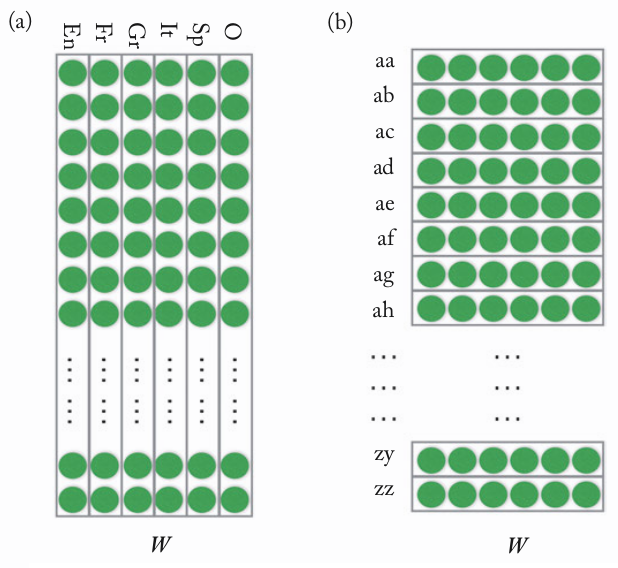
\includegraphics[scale=0.35]{pics/2rep.png}
\end{figure}

Two views of the $W$ matrix. (a) Each column corresponds to a language. (b) Each row
corresponds to a letter bigram. Source: \cite{goldberg2017neural}.


\end{itemize}
\end{scriptsize}
\end{frame}



\begin{frame}{Representations}

\begin{scriptsize}
\begin{itemize}
\item A column of $W$ can be taken to be a $784$-dimensional vector representation of a language in terms of its characteristic letter-bigram patterns.
\item We can then cluster the 6 language vectors according to their similarity.
\item Each of the 784 rows of $W$ provide a 6-dimensional vector representation of that bigram in terms of the languages it prompts.

\end{itemize}
\end{scriptsize}
\end{frame}


\begin{frame}{Representations}

\begin{scriptsize}
\begin{itemize}
\item Representations are central to deep learning.
\item One could argue that the main power of deep-learning is the ability to learn good representations.
\item In the linear case, the representations are interpretable.
\item We can assign a meaningful interpretation to each dimension in the
representation vector.
\item For example: each dimension corresponds to a particular language or letter-bigram.
\end{itemize}
\end{scriptsize}
\end{frame}


\begin{frame}{Representations}

\begin{scriptsize}
\begin{itemize}
\item Deep learning models, on the other hand,  often learn a cascade of representations of the input that build on top of each other. 
\item These representations are often not interpretable.
\item We do not know which properties of the input they capture.
\item However, they are still very useful for making predictions.
\end{itemize}
\end{scriptsize}
\end{frame}

\begin{frame}{One-Hot Vector Representation}

\begin{scriptsize}
\begin{itemize}
\item The input vector $\vec{x}$ in our language classification example contains the normalized bigram counts in the document $D$.
\item This vector can be decomposed into an average of $|D|$ vectors, each corresponding to a particular document position $i$:
\begin{equation}
 \vec{x} = \frac{1}{|D|} \sum_{i=1}^{|D|} \vec{x}^{D_{[i]}}
\end{equation}
\item Here, $D_{[i]}$ is the bigram at document position $i$.
\item Each vector  $\vec{x}^{D_{[i]}} \in \mathcal{R}^{784}$ is a one-hot vector.
\end{itemize}
\end{scriptsize}
\end{frame}

\begin{frame}{One-Hot Vector Representation}

\begin{scriptsize}
\begin{itemize}
\item A one-hot vector: all entries are zero except the single entry corresponding to the letter bigram $D_{[i]}$, which is 1.
\item The resulting vector $\vec{x}$ is commonly referred to as an averaged bag of bigrams (more generally averaged bag of words , or just bag of words).
\item Bag-of-words (BOW) representations contain information about the identities of all the ``words'' (here, bigrams) of the document, without considering their order.
\item A one-hot representation can be considered as a bag-of-a-single-word.
\end{itemize}
\end{scriptsize}
\end{frame}



\begin{frame}{One-Hot Vector Representation}

\begin{scriptsize}

\begin{figure}[htb]
	\centering
	 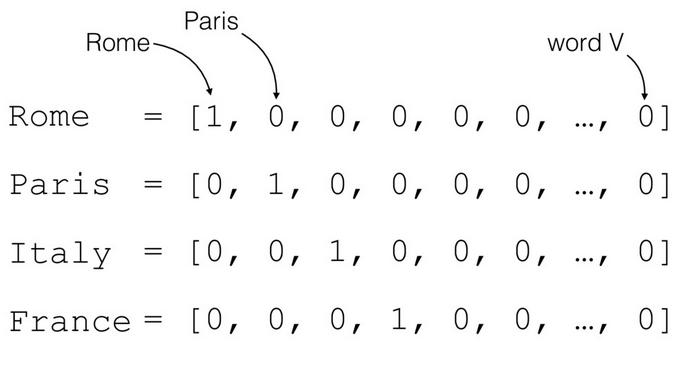
\includegraphics[scale=0.35]{pics/onehot.png}
\end{figure}

One-hot vectors of words. Source: \url{https://medium.com/@athif.shaffy/one-hot-encoding-of-text-b69124bef0a7}.

\end{scriptsize}
\end{frame}


\begin{frame}{Log-linear Multi-class Classification}

\begin{scriptsize}
\begin{itemize}
\item In the binary case, we transformed the linear prediction into a probability estimate by passing it through the sigmoid function, resulting in a log-linear model.
\item The analog for the multi-class case is passing the score vector through the \textbf{softmax} function:
\begin{equation}
 \operatorname{softmax}(\vec{x})_{[i]} = \frac{e^{\vec{x}_{[i]}}}{\sum_j e^{\vec{x}_{[j]}}}
\end{equation}
Resulting in:
\begin{equation}
\begin{split}
\hat{\vec{y}} \quad & =  \operatorname{softmax}(\vec{x} \cdot W + \vec{b})  \\
\hat{\vec{y}}_{[i]} \quad & = \frac{e^{(\vec{x} \cdot W + \vec{b})_{[i]}}}{\sum_j e^{(\vec{x} \cdot W + \vec{b})_{[j]}}}
\end{split}
\end{equation}
\item The softmax transformation forces the values in $\hat{\vec{y}}$ to be positive and sum to 1, making them interpretable as a probability distribution.
\end{itemize}
\end{scriptsize}
\end{frame}

\begin{frame}{Limitations of linear models: the XOR problem}
\begin{scriptsize}
\begin{itemize}
\item The hypothesis class of linear (and log-linear) models is severely restricted.
\item For example, it cannot represent the XOR function, defined as:
\begin{equation}
 \begin{split}
  \operatorname{xor}(0,0) \quad & = 0 \\
  \operatorname{xor}(1,0) \quad & = 1 \\
  \operatorname{xor}(0,1) \quad & = 1 \\
  \operatorname{xor}(1,1) \quad & = 0 \\
 \end{split}
\end{equation}
\end{itemize}
\end{scriptsize}
\end{frame}


\begin{frame}{Limitations of linear models: the XOR problem}
\begin{scriptsize}
\begin{itemize}
\item There is no parameterization $\vec{w} \in \mathcal{R}^2, b \in \mathcal{R}$ such that:
\begin{equation}
 \begin{split}
  (0,0) \cdot \vec{w} +b \quad & < 0 \\
  (0,0) \cdot \vec{w} +b \quad & < 0 \\
  (0,0) \cdot \vec{w} +b \quad & < 0 \\
  (0,0) \cdot \vec{w} +b \quad & < 0 \\
 \end{split}
\end{equation}
\end{itemize}
\end{scriptsize}
\end{frame}



\begin{frame}{Limitations of linear models: the XOR problem}
\begin{scriptsize}
\begin{itemize}
\item To see why, consider the following plot of the XOR function, where blue Os denote the positive class and green Xs the negative class.
\begin{figure}[htb]
	\centering
	 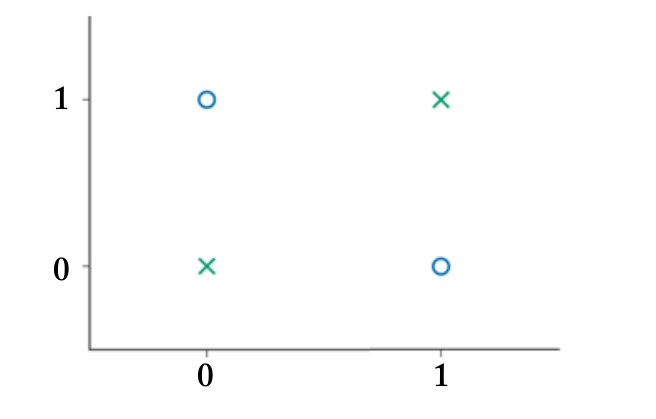
\includegraphics[scale=0.35]{pics/xor.png}
\end{figure}
\item It is clear that no straight line can separate the two classes.
\end{itemize}
\end{scriptsize}
\end{frame}




\begin{frame}{Nonlinear input transformations}
\begin{scriptsize}
\begin{itemize}
\item If we transform the points by feeding each of them through the nonlinear function $\phi(x_1,x_2) = [x_1 \times x_2, x_1 x_2 ]$ , the XOR problem becomes linearly separable.
\begin{figure}[htb]
	\centering
	 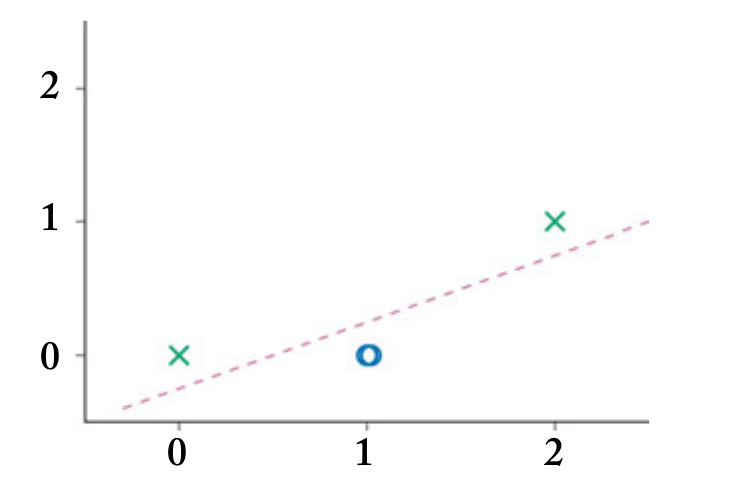
\includegraphics[scale=0.25]{pics/xor2.png}
\end{figure}

\item The function $\phi$ mapped the data into a representation that is suitable for linear classification.

\end{itemize}
\end{scriptsize}
\end{frame}


\begin{frame}{Nonlinear input transformations}
\begin{scriptsize}
\begin{itemize}
\item We can now easily train a linear classifier to solve the XOR problem.
\begin{equation}
 \hat{y} = f(\vec{x}) = \phi(\vec{x}) \cdot \vec{w} +b
\end{equation}
\item Problem: we need to manually define the function $\phi$.
\item This process is dependent on the particular dataset, and requires a lot of human intuition.
\item Solution: define a trainable nonlinear mapping function, and train it in con-
junction with the linear classifier.
\item Finding the suitable representation becomes the responsibility of the training algorithm.
\end{itemize}
\end{scriptsize}
\end{frame}


\begin{frame}{Trainable mapping functions}
\begin{scriptsize}
\begin{itemize}
\item The mapping function can take the form of a parameterized linear model.
\item Followed by a nonlinear activation function $g$ that is applied to each of the output dimensions:
\begin{equation}
\begin{split}
\hat{y} = f(\vec{x}) = \phi(\vec{x}) \cdot \vec{w} +b \\
\phi(\vec{x}) = g(\vec{x}W'+ \vec{b}') \\
\end{split} 
\end{equation}
\end{itemize}
\end{scriptsize}
\end{frame}



\begin{frame}{Trainable mapping functions}
\begin{scriptsize}
\begin{itemize}
\item By taking $g(x) = \operatorname{max}(0, x)$ and $W' = \begin{pmatrix}
    1 & 1 \\ 1 & 1 \end{pmatrix}$, $\vec{b}' = \begin{pmatrix}
    -1 & 0 \end{pmatrix}$.
\item We get an equivalent mapping to $[x_1 \times x_2, x_1 + x_2]$  for the our points of interest (0,0), (0,1), (1,0), and (1,1).
\item This successfuly solves the XOR problem!
\item Learning both the representation function and the linear classifier on top of it at the same time is the main idea behind deep learning and neural networks.
\item In fact, previous equation describes a very common neural network architecture called a multi-layer perceptron (MLP).
\end{itemize}
\end{scriptsize}
\end{frame}




\begin{frame}
\frametitle{Questions?}
%\vspace{1.5cm}
\begin{center}\LARGE Thanks for your Attention!\\ \end{center}



\end{frame}

\begin{frame}[allowframebreaks]\scriptsize
\frametitle{References}
\bibliography{bio}
\bibliographystyle{apalike}
%\bibliographystyle{flexbib}
\end{frame}  


%%%%%%%%%%%%%%%%%%%%%%%%%%%

\end{document}
